\clearpage
\section{Model Optimization}

\subsection{Problem 1 Optimization}
From previous training, we learned that the time complexity is particularly high for the SVM algorithm. The process of training the model takes a lot of time due to the overfitting phenomenon and the intricacy of the dataset, while the accuracy rate is hovering at 45\%. By adjusting the parameters respectively, we can have a better view of how to optimize the model to get higher accuracy.
\subsubsection{Impact of The Number of Training Samples on Accuracy}
We assign kernel = 'linear', set other parameters as default. By changing different size of training samples, we obtain the accuracy respectively as shown in Figure \ref{Impact of the number of training samples on accuracy for problem 1}.
\begin{figure}[h!]
    \centering
    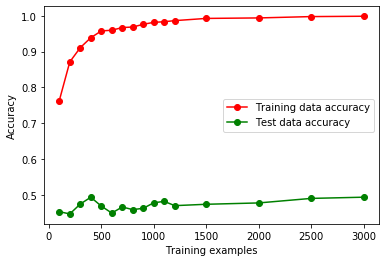
\includegraphics[scale=0.6]{figures/Impact of the number of training samples on accuracy for problem 1.png}
    \caption{Impact of the number of training samples on accuracy for problem 1}
    \label{Impact of the number of training samples on accuracy for problem 1}
\end{figure}

As the number of the training data increases, the training data accuracy increases as well and flattened.


Further analysis show that when kernel = 'linear', and the number of training samples is 400, the optimal accuracy is 49.30\%.
\subsubsection{Impact of The Kernel Function on Accuracy}
We tested four kinds of kernels: linear, rbf, poly and sigmoid. The accuracies are shown in the Figure \ref{fig:Impact of the kernel on accuracy for problem 1}.
\begin{figure}[h]
    \centering
    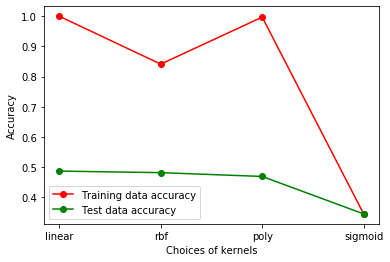
\includegraphics[scale=0.6]{figures/Impact of the kernel on accuracy for problem 1.png}
    \caption{Impact of the kernel on accuracy for problem 1}
    \label{fig:Impact of the kernel on accuracy for problem 1}
\end{figure}

The accuracy obtained by the linear kernel and the polynomial kernel is relatively close, while the sigmoid kernel offered poor performance.
\subsubsection{Detailed Parameters Adjustments of Kernel Radial Basis Function(rbf)}
Here, we would like to go far into the case of kernel 'rbf', to find out how the rbf kernel performs under different parameters C and $\gamma$. 


By setting the size of training data at 400 and adjusting C and $\gamma$ respectively, the ouput accuracies are shown in the Table \ref{table:Accuracy of different C and gamma of rbf kernel} and Figure \ref{fig:Accuracy of different C and gamma of rbf kernel}. We select C = [0.1, 1, 2, 3, 4, 5,6, 7, 9, 11] and $\gamma$ = [0.00001, 0.0001, 0.01].

\begin{table}[h!]
\centering
\begin{tabular}{||c| c | c | c||} 
 \hline
 \textbf{C} & \textbf{$\gamma$=0.00001} & \textbf{$\gamma$=0.0001} & \textbf{$\gamma$=0.01} \\ [0.5ex] 
 \hline\hline
0.1 & 0.329703 & 0.329703 & 0.329703\\\hline
1 & 0.329703 & 0.460627 & 0.329703\\\hline
2 & 0.329703 & 0.464822	& 0.335443\\\hline
3 & 0.424934 & 0.482043	& 0.336032\\\hline
4 & 0.420812 & 0.517883	& 0.335369\\\hline
5 & 40.42957 & 0.521195	& 0.335369\\\hline
6 & 50.398366 & 0.519797 & 0.335369\\\hline
7 & 60.39844 & 0.518104	& 0.335369\\\hline
9 & 70.45577 & 0.514645	& 0.335369\\\hline
11 & 90.472917& 0.520459 & 0.335369\\[1ex] 
 \hline
\end{tabular}
\caption{Accuracy of different C and $\gamma$ of rbf kernel}
\label{table:Accuracy of different C and gamma of rbf kernel}
\end{table}

\begin{figure}[h!]
    \centering
    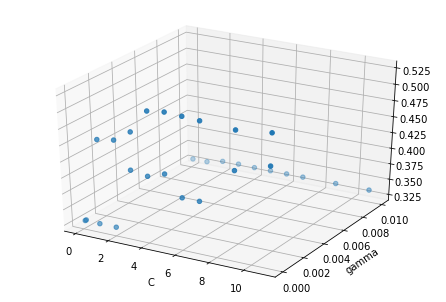
\includegraphics[scale=0.4]{figures/Accuracy of different C and gamma of rbf kernel.png}
    \caption{Accuracy of different C and gamma of rbf kernel}
    \label{fig:Accuracy of different C and gamma of rbf kernel}
\end{figure}

From the Table \ref{table:Accuracy of different C and gamma of rbf kernel} and Figure \ref{fig:Accuracy of different C and gamma of rbf kernel} and our further testing, we can conclude that when training size = 1200,  C = 6.0, $\gamma$ = 0.0001, the test data has a highest accuracy of 57.81\%, which is close to the highest accuracy obtained by the linear kernel.
\subsection{Problem 2 Optimization}

\subsubsection{Impact of The Total Number of Training Samples and The Size of Sub-Groups on Accuracy}
Assigned linear kernel, we set different size of training samples and different size of sub-groups to test how they influence the final accuracy. The size of training samples is designated respectively as [330, 600, 900, 1200, 1600, 2000, 3000, 4000, 5000, 6000, 8000, 10000], and the size of sub-groups is designated respectively as [20, 40, 60, 80].

\begin{table}[h!]
\centering
\begin{tabular}{||c  c || c  c  c c ||} 
\hline
&  & \multicolumn{4}{c||}{\textbf{The size of sub-group}}\\ [0.5ex] 
& & 20 & 40 & 60 & 80 \\\hline\hline
\multirow{12}{8em}{\textbf{The size of training sample}} & 330   & 0.4808 & 0.5394 & 0.5394 & 0.4429\\
& 600   & 0.5258 & 0.5664 & 0.4962 & 0.4287\\
& 900   & 0.5076 & 0.4725 & 0.5399 & 0.5190\\
& 1200  & 0.4981 & 0.5753 & 0.5388 & 0.5333\\
& 1600  & 0.5077 & 0.5073 & 0.5204 & 0.4870\\
& 2000  & 0.5789 & 0.5448 & 0.5394 & 0.5012\\
& 3000  & 0.5098 & 0.5187 & 0.5094 & 0.5176\\
& 4000  & 0.5568 & 0.5391 & 0.5483 & 0.5123\\
& 5000  & 0.5286 & 0.4511 & 0.4823 & 0.5217\\
& 6000  & 0.5237 & 0.5239 & 0.5367 & 0.5036\\
& 8000  & 0.5061 & 0.4614 & 0.4538 & 0.5025\\
& 10000 & 0.5086 & 0.5198 & 0.4895 & 0.4848\\[1ex] 
\hline
\end{tabular}
\caption{The impact of the size of training samples and the size of sub-groups on accuracy}
\label{table:The impact of the size of training samples and the size of sub-groups on accuracy}
\end{table}

From Table \ref{table:The impact of the size of training samples and the size of sub-groups on accuracy}. and our further testing, the highest accuracy 62.1\% occurs when the size of training samples is 1200 and the size of sub-groups is 30.

\subsubsection{Impact of The Kernel Function on Accuracy}
Same as problem 1, we set four kernels: linear, rbf, poly and sigmoid. The accuracies of these four kernel are shown in Figure \ref{fig:The accuracy of different kernels}.
\begin{figure}[h!]
    \centering
    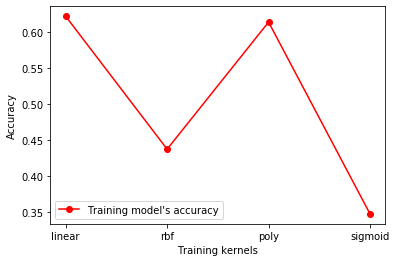
\includegraphics[scale=0.6]{figures/The accuracy of different kernels.png}
    \caption{The accuracy of different kernels}
    \label{fig:The accuracy of different kernels}
\end{figure}


As shown in the Figure \ref{fig:The accuracy of different kernels}, the linear and rbf kernel have similar values, while the rbf and sigmoid kernel do not behave as good as the previous two kernels.

\subsubsection{Detailed Parameters Adjustments of Kernel Radial Basis Function(rbf)}
Same as problem 1, we assign rbf kernel. Meanwhile, adjust the value of C and $\gamma$, to test how these two parameters influence the final accuracy.
We set C =  [0.1, 1, 2, 3, 4, 5, 6, 7, 9, 11], $\gamma$ = [0.00001, 0.0001, 0.01] for cross validation.
The results are shown in Table \ref{table:The accuracy of different C and gamma for rbf kernel} and Figure \ref{Impact of different C and gamma on the accuracy of rbf kernel}. 

\begin{table}[h!]
\centering
\begin{tabular}{||c| c | c | c||} 
 \hline
 \textbf{C} & \textbf{$\gamma$=0.00001} & \textbf{$\gamma$=0.0001} & \textbf{$\gamma$=0.01} \\ [0.5ex] 
 \hline\hline
0.1 & 0.4561 & 0.5483 & 0.4217\\\hline 
1 & 0.4427 & 0.4566 & 0.4561\\\hline 
2 & 0.4125 & 0.4561 & 0.5425\\\hline 
3 & 0.4561 & 0.5776 & 0.4204\\\hline 
4 & 0.4532 & 0.4325 & 0.4707\\\hline 
5 & 0.4294 & 0.4561 & 0.5419\\\hline 
6 & 0.4561 & 0.5562 & 0.4277\\\hline 
7 & 0.5578 & 0.4223 & 0.4722\\\hline 
9 & 0.4296 & 0.4561 & 0.5452\\\hline 
11 & 0.4561 & 0.5569 & 0.4335\\[1ex] 
 \hline
\end{tabular}
\caption{The accuracy of different C and $\gamma$ for rbf kernel}
\label{table:The accuracy of different C and gamma for rbf kernel}
\end{table}

\begin{figure}[h!]
    \centering
    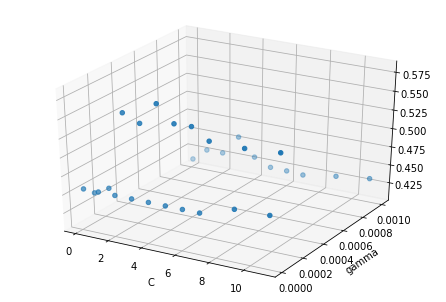
\includegraphics[scale=0.5]{figures/Impact of different C and gamma on the accuracy of rbf kernel.png}
    \caption{Impact of different C and $\gamma$ on the accuracy of rbf kernel}
    \label{Impact of different C and gamma on the accuracy of rbf kernel}
\end{figure}

From Table \ref{table:The accuracy of different C and gamma for rbf kernel} and Figure \ref{Impact of different C and gamma on the accuracy of rbf kernel}, it can be concluded that the perferable parameter C for rbf kernel should be 3.0 and $\gamma$ should be 0.0001. 